% Created 2022-09-27 Di 12:32
% Intended LaTeX compiler: xelatex
\documentclass[presentation]{beamer}
\usepackage{graphicx}
\usepackage{longtable}
\usepackage{wrapfig}
\usepackage{rotating}
\usepackage[normalem]{ulem}
\usepackage{amsmath}
\usepackage{amssymb}
\usepackage{capt-of}
\usepackage{hyperref}
\usetheme{default}
\author{Persentor: Silin Zhao Supervisor: Patrick Michaelis}
\date{\today}
\title{Report oft Practical Course on High-Performance Computing}
\subtitle{ Parallel Deep Learning pipelines using Go and MPI }
\hypersetup{
 pdfauthor={Persentor: Silin Zhao Supervisor: Patrick Michaelis},
 pdftitle={Report oft Practical Course on High-Performance Computing},
 pdfkeywords={},
 pdfsubject={},
 pdfcreator={Emacs 28.2 (Org mode 9.5.5)}, 
 pdflang={English}}
\begin{document}

\maketitle
\begin{frame}[label={sec:org59bb5fb}]{Project notation}
\begin{block}{Youtube link}
\url{https://www.youtube.com/watch?v=2siZQBvRPuY\&t=6s}
\end{block}
\begin{block}{Datasets}
\begin{itemize}
\item This project source code can be found \url{https://github.com/scofild429/go\_mpi\_network},This is the \textbf{README} page.
\item Iris dataset (\url{https://www.kaggle.com/datasets/saurabh00007/iriscsv})
\item Intel image classification, (\url{https://www.kaggle.com/datasets/puneet6060/intel-image-classification?resource=download}). Download it,  put archive it in the folder ./datasets/
\end{itemize}

\textbf{All training data will equally divied for each training network, specially for mpi}
\end{block}
\end{frame}

\begin{frame}[label={sec:orgc6ef77f},fragile]{Configuration  example}
 \begin{itemize}
\item ./goai/.irisenv
\item ./goai/.imgenv
\end{itemize}
\begin{verbatim}
inputdataDims=4
inputLayerNeurons=30
hiddenLayerNeurons=20
outputLayerNeurons=3
labelOnehotDims=3
numEpochs=100
learningRate=0.01
batchSize=4
\end{verbatim}
\end{frame}

\begin{frame}[label={sec:org68361bb},fragile]{Sumbit the job in cluster}
 \textbf{no singularity}, installing golang 1.18 was failed always

using binary executable code of golang, \textbf{go build}

\begin{verbatim}
#!/bin/bash
#SBATCH --job-name mpi-go-neural-network
#SBATCH -N 1
#SBATCH -p fat
#SBATCH -n 20
#SBATCH --time=01:30:00

module purge
module load openmpi

mpirun -n 20 ./goai
\end{verbatim}
\end{frame}

\begin{frame}[label={sec:orge3da525}]{Deep learning's problem}
As AI comes to deep learning, the computing resource becomes more critical for training process.

\textbf{Applications:}
\begin{itemize}
\item Image Classification
\item NLP
\item Semantic segmentation
\end{itemize}

\textbf{Solution}
\begin{itemize}
\item GPU
\item TPU
\item \textbf{Distributed learning}
\end{itemize}
\end{frame}

\begin{frame}[label={sec:org22d3c14},fragile]{Single network architecture}
 \begin{verbatim}
raining data -> inputLayer(w1, b1) -> dinputLayer
Normalization
dinputLayer -> hiddenLayer(w2, b2) -> dhiddenLayer
Normalization
dhiddenLayer -> OutputLayer(w3, b3) -> doutputLayer
\end{verbatim}
Loss = L2: (doutputLayer - onehotlable)\textsuperscript{2}
\begin{verbatim}
Backpropagation from Loss  of Outputlayer  to w3, b3
Backpropagation from error of Hiddenlayer  to w2, b2
Backpropagation from error of Inputlayer   to w1, b1
\end{verbatim}

Derivative of sigmoid, Normalization, Standardization

\begin{itemize}
\item Stochastic Gradient Descent (SGD)
\item Mini-batch Gradient Descent (MBGD)
\item Batch Gradient Descent (BGD)
\end{itemize}
\end{frame}

\begin{frame}[label={sec:orgaf239ea}]{Illustration of weights updating}
\begin{center}
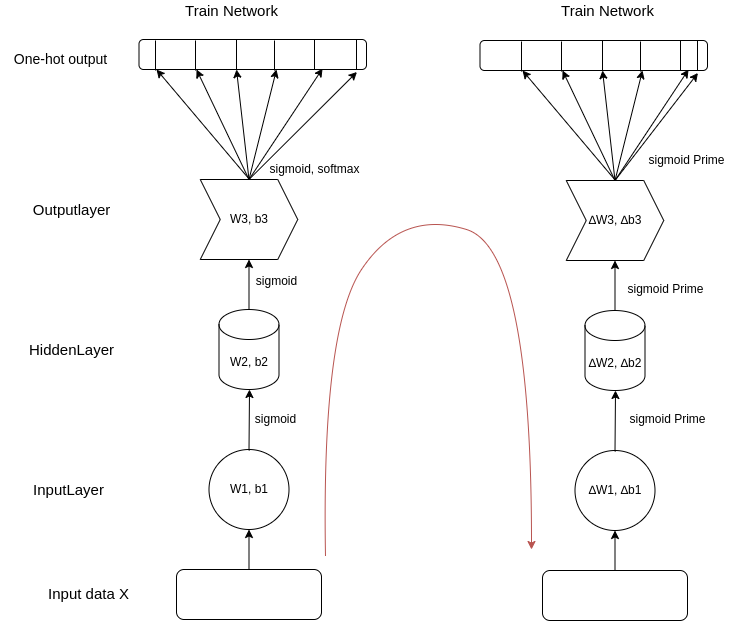
\includegraphics[width=0.8\textwidth]{./png/NeuralNetwork.png}
\end{center}
\end{frame}

\begin{frame}[label={sec:orga939ba6},fragile]{Code implementation}
 \begin{verbatim}
func main() {
	singlenode.Single_node_iris(true)
	mpicode.Mpi_iris_Allreduce()
	mpicode.Mpi_iris_SendRecv()
	mpicode.Mpi_images_Allreduce()
	mpicode.Mpi_images_SendRecv()
}
\end{verbatim}

You can review my code, and choose one of them to be executed in /goai/myai.go main function.

Comparing with python:

\begin{itemize}
\item ./pytorchDemo/irisfromscratch.py
\item ./pytorchDemo/iriswithpytorch.py
\item ./pytorchDemo/logisticRcuda.py
\end{itemize}
\end{frame}

\begin{frame}[label={sec:orgfee0999}]{Network performance(iris dataset)}
\begin{columns}
\begin{column}{0.6\columnwidth}
\begin{block}{Loss}
\begin{center}
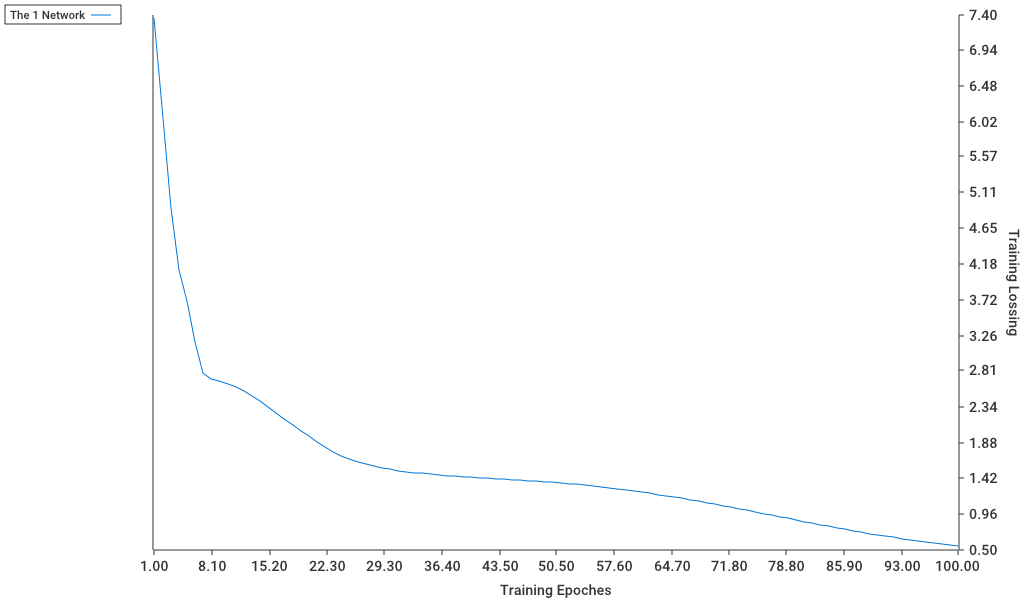
\includegraphics[width=.9\linewidth]{./png/single_node_loss.png}
\end{center}
\end{block}
\end{column}

\begin{column}{0.6\columnwidth}
\begin{block}{Accuarcy}
\begin{center}
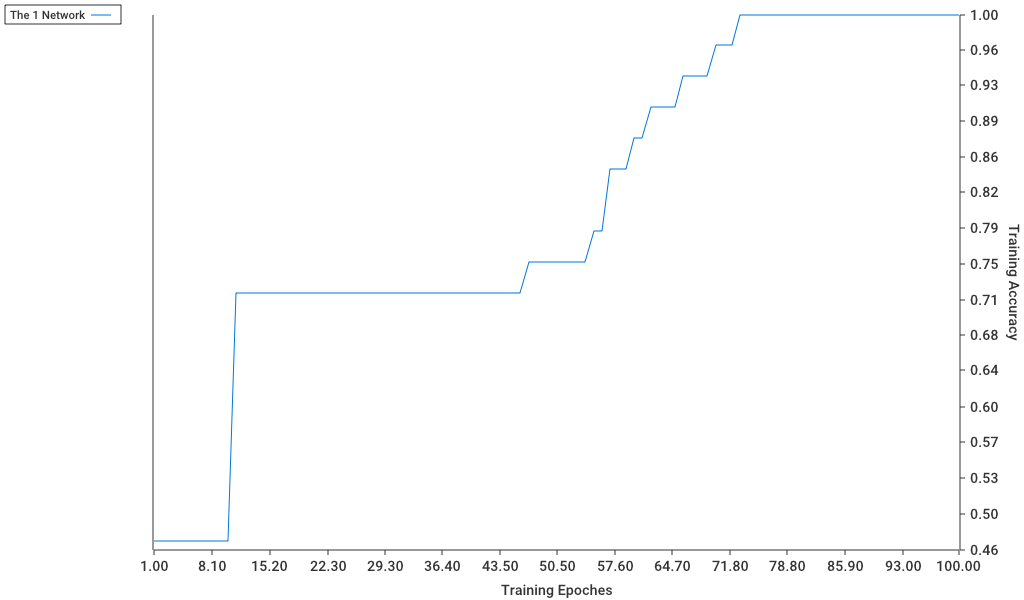
\includegraphics[width=.9\linewidth]{./png/single_node_acc.png}
\end{center}
\end{block}
\end{column}
\end{columns}
\end{frame}

\begin{frame}[label={sec:orgcef7e89},fragile]{MPI communication}
 \begin{verbatim}
github.com/sbromberger/gompi
import CGO as C
\end{verbatim}

\begin{itemize}
\item \textbf{Collective}
\begin{itemize}
\item gompi.BcastFloat64s() -> C.MPI \textunderscore Bcast()
\item gompi.AllreduceFloat64s -> C.MPI \textunderscore Allreduce()
\end{itemize}

\item \textbf{Non Collective}
\begin{itemize}
\item gompi.SendFloat64s() -> C.MPI \textunderscore Send()
\item gompi.SendFloat64() -> C.MPI \textunderscore Send()
\item gompi.RecvFloat64s() -> C.MPI \textunderscore Recv()
\item gompi.RecvFloat64() -> C.MPI \textunderscore Recv()
\end{itemize}
\end{itemize}
\end{frame}

\begin{frame}[label={sec:org576e8a6}]{Non collective architecture}
\begin{center}
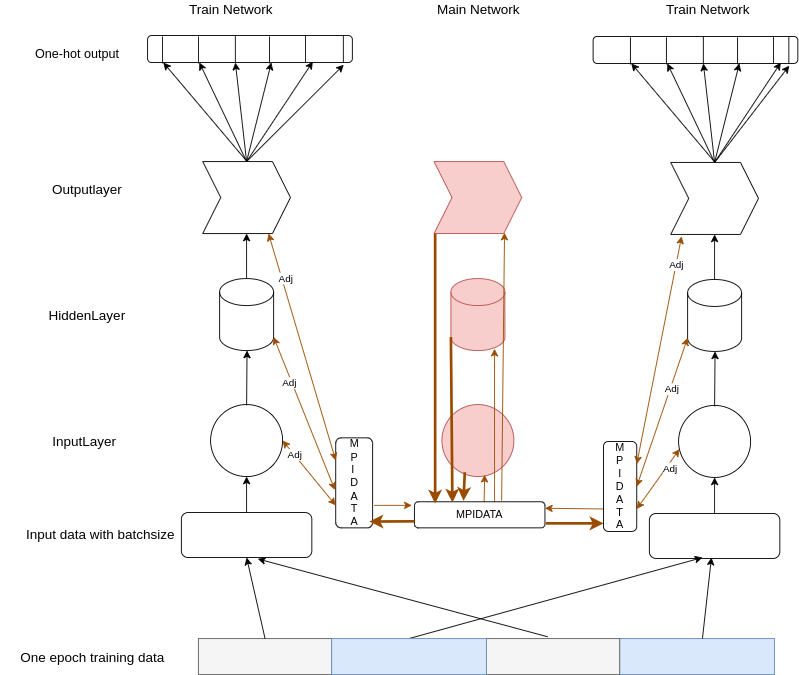
\includegraphics[width=0.8\textwidth]{./png/MPINetworkSendRecv.png}
\end{center}
\end{frame}

\begin{frame}[label={sec:orge9806fb}]{Non collective design}
\begin{block}{rank = 0}
\begin{itemize}
\item in \textbf{main network} weights will be initialized, but not for training,
\item weights will broadcast to all other training networks
\end{itemize}
\end{block}
\begin{block}{rank != 0}
\begin{itemize}
\item in \textbf{train network} receive weights from main network for initialization
\item After each batch training done, sending its weights variance to main network
\end{itemize}
\end{block}
\begin{block}{rank = 0}
\begin{itemize}
\item receiving the  variance from all training network
\item accumulating and then sending back to training network
\end{itemize}
\end{block}
\begin{block}{rank != 0}
\begin{itemize}
\item start next training batch
\end{itemize}
\end{block}
\end{frame}

\begin{frame}[label={sec:orgf132af2}]{Collective architecture}
\begin{center}
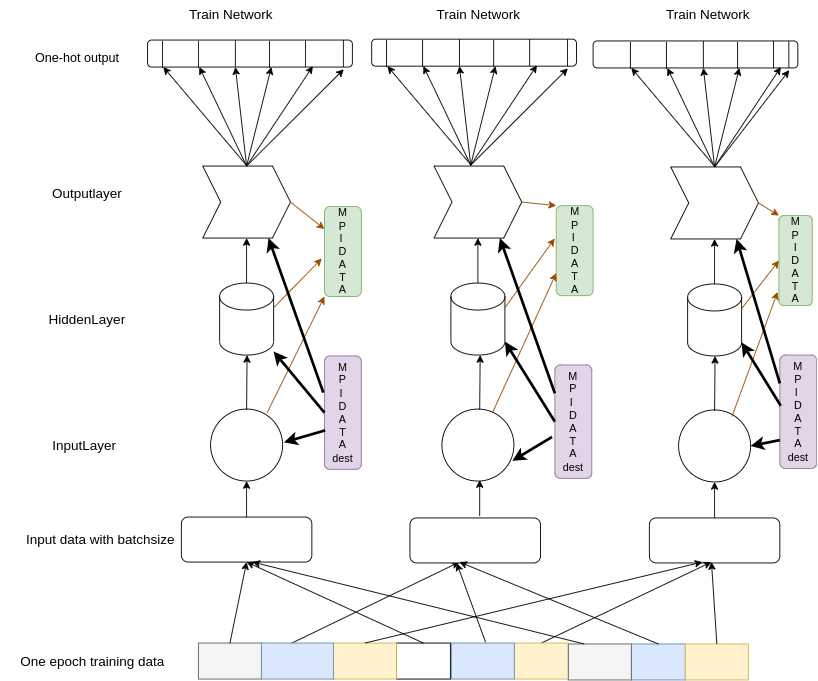
\includegraphics[width=0.8\textwidth]{./png/MPINetworkAllreduce.png}
\end{center}
\end{frame}
\begin{frame}[label={sec:orgb162896}]{Collective design}
\begin{itemize}
\item All network train its data respectively,
\item After each train batch, pack all weights into array
\item MPI\textsubscript{Allreduce} for new array
\item updating weights with  new array
\end{itemize}
\end{frame}

\begin{frame}[label={sec:org3f3cba4}]{Iris dataset performance for non-collective}
\begin{columns}
\begin{column}{0.6\columnwidth}
\begin{block}{Send\&Recv loss}
\begin{center}
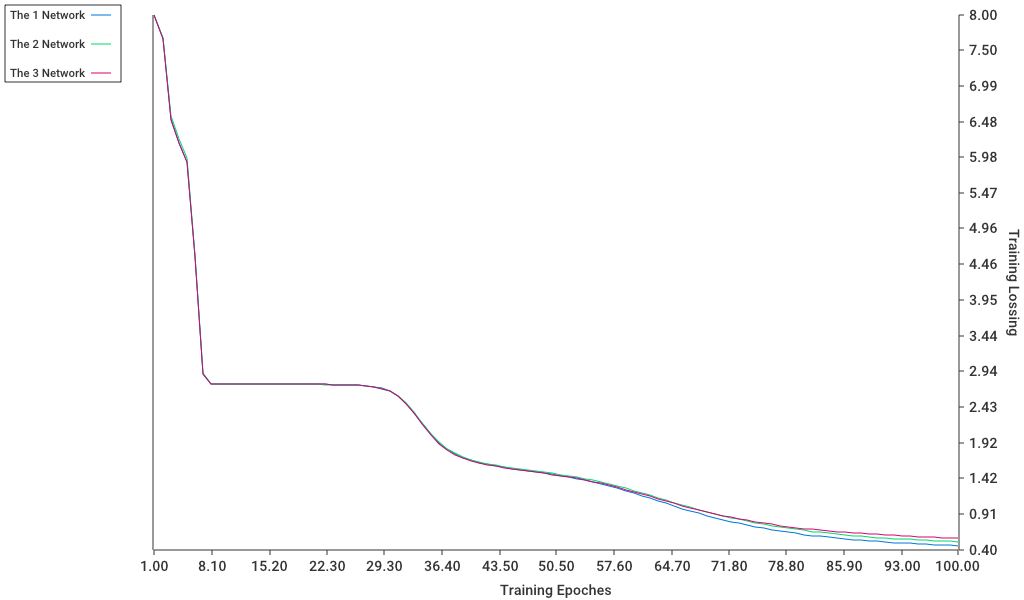
\includegraphics[width=.9\linewidth]{./png/iris_sendrecv_loss.png}
\end{center}
\end{block}
\end{column}

\begin{column}{0.6\columnwidth}
\begin{block}{Send\&Recv accuracy}
\begin{center}
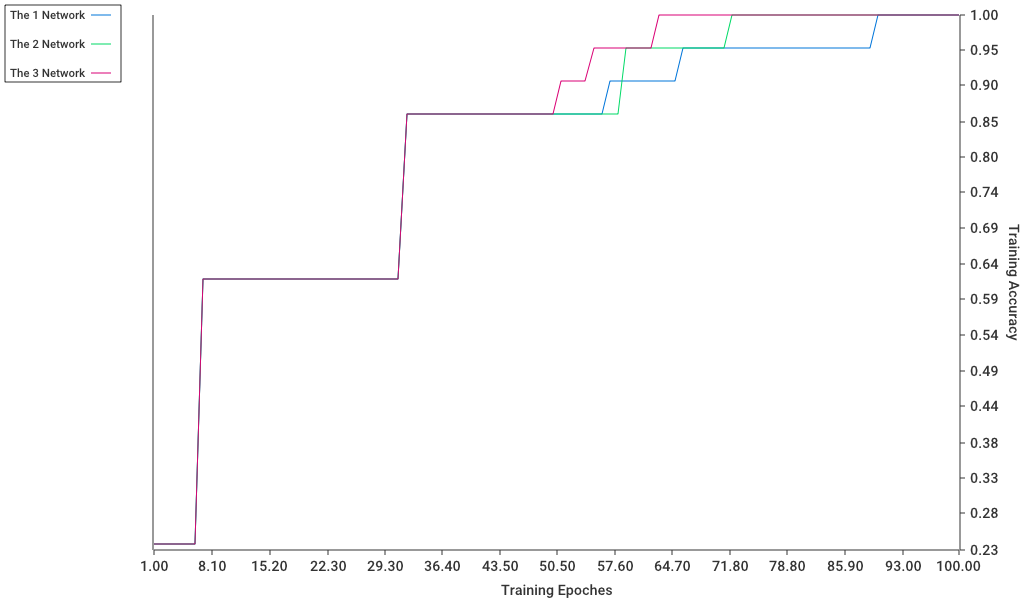
\includegraphics[width=.9\linewidth]{./png/iris_sendrecv_accuracy.png}
\end{center}
\end{block}
\end{column}
\end{columns}
\end{frame}

\begin{frame}[label={sec:org1c71325}]{Iris dataset performance for collective}
\begin{columns}
\begin{column}{0.6\columnwidth}
\begin{block}{Allreduce loss}
\begin{center}
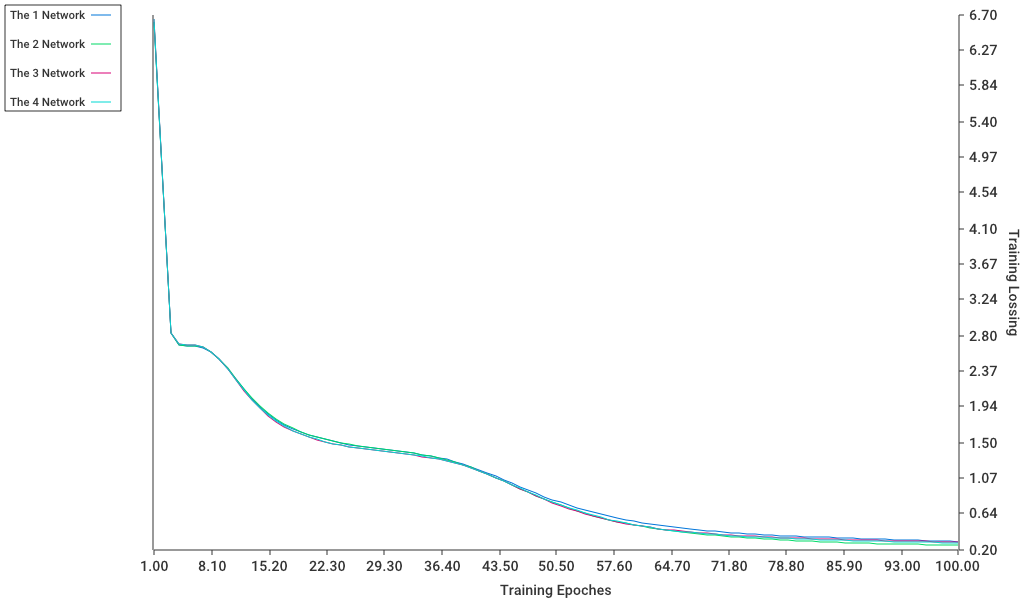
\includegraphics[width=.9\linewidth]{./png/iris_allreduce_loss.png}
\end{center}
\end{block}
\end{column}
\begin{column}{0.6\columnwidth}
\begin{block}{Allreduce accuracy}
\begin{center}
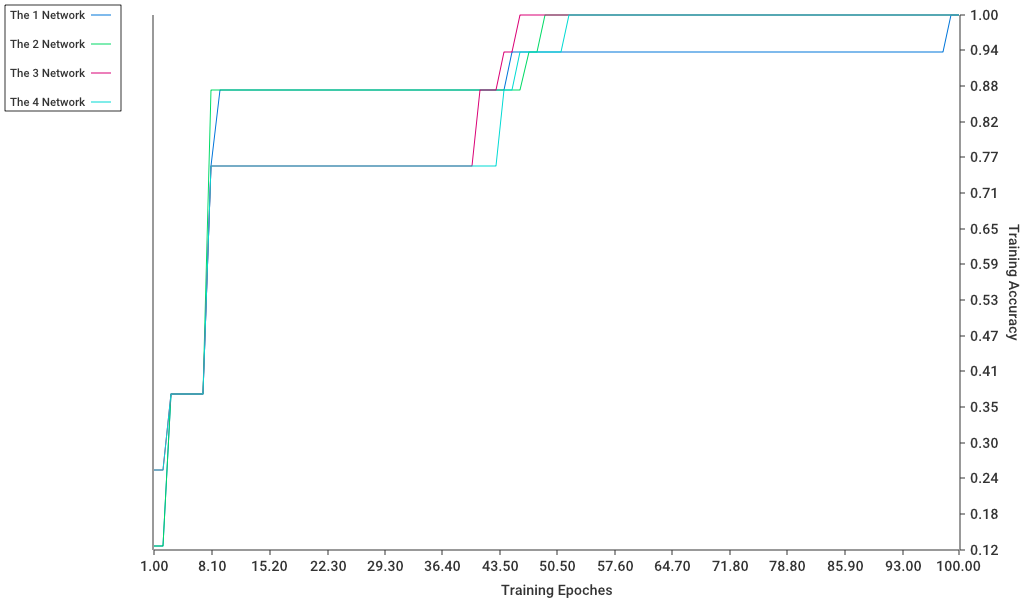
\includegraphics[width=.9\linewidth]{./png/iris_allreduce_accuracy.png}
\end{center}
\end{block}
\end{column}
\end{columns}
\end{frame}

\begin{frame}[label={sec:orgfb39063}]{Intel image classification performance}
\begin{columns}
\begin{column}{0.55\columnwidth}
\begin{block}{Send\&Recv loss (220 images)}
\begin{center}
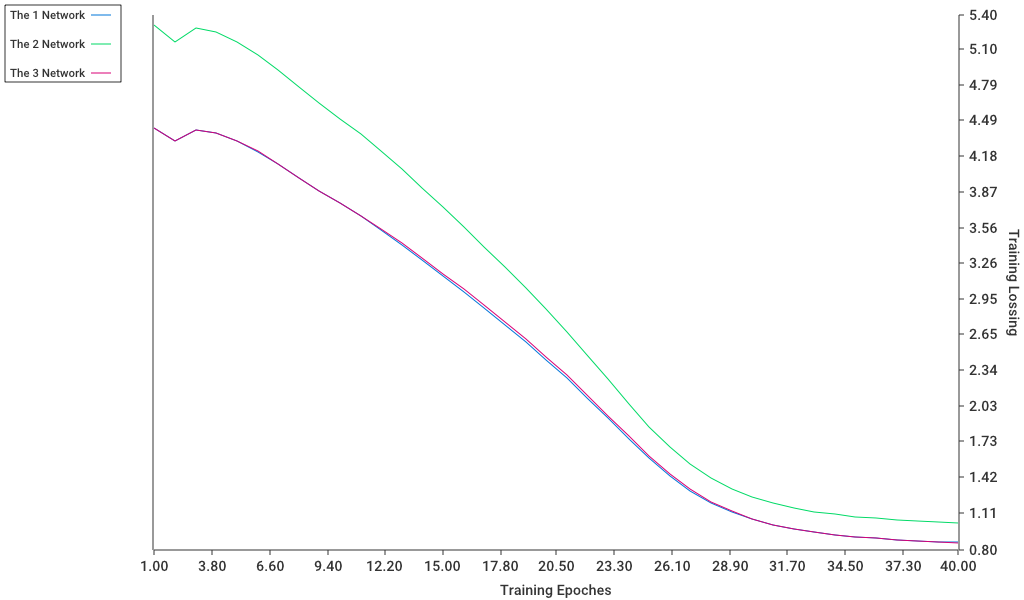
\includegraphics[width=.9\linewidth]{./png/intelImage_subset_sendrecving_loss.png}
\end{center}
 SendRecv loss (14000 images)
\begin{center}
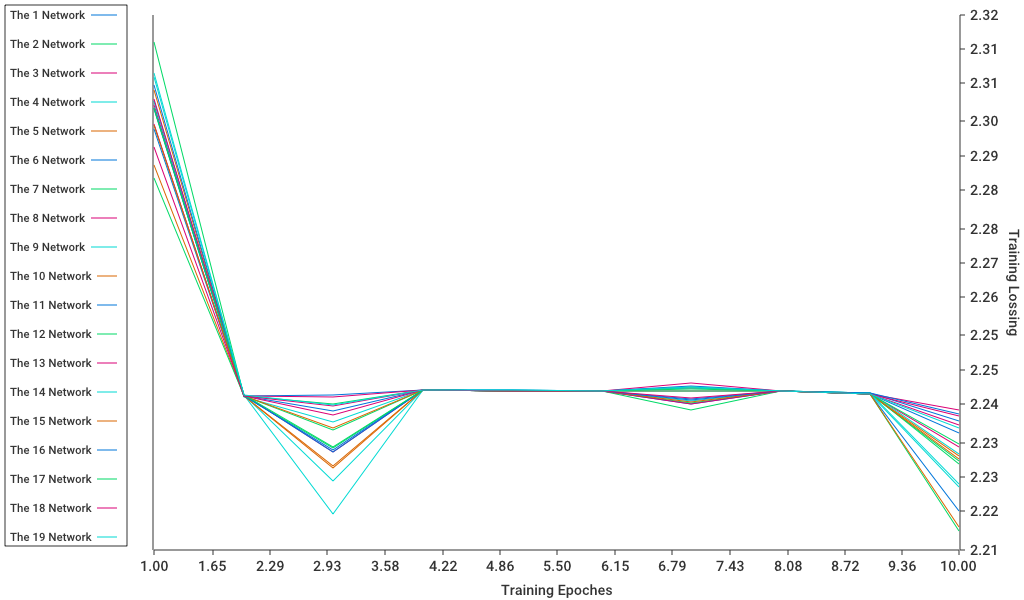
\includegraphics[width=.9\linewidth]{./png/intelImage_sendrecv_loss.png}
\end{center}
\end{block}
\end{column}
\begin{column}{0.55\columnwidth}
\begin{block}{Allreduce loss (220 images)}
\begin{center}
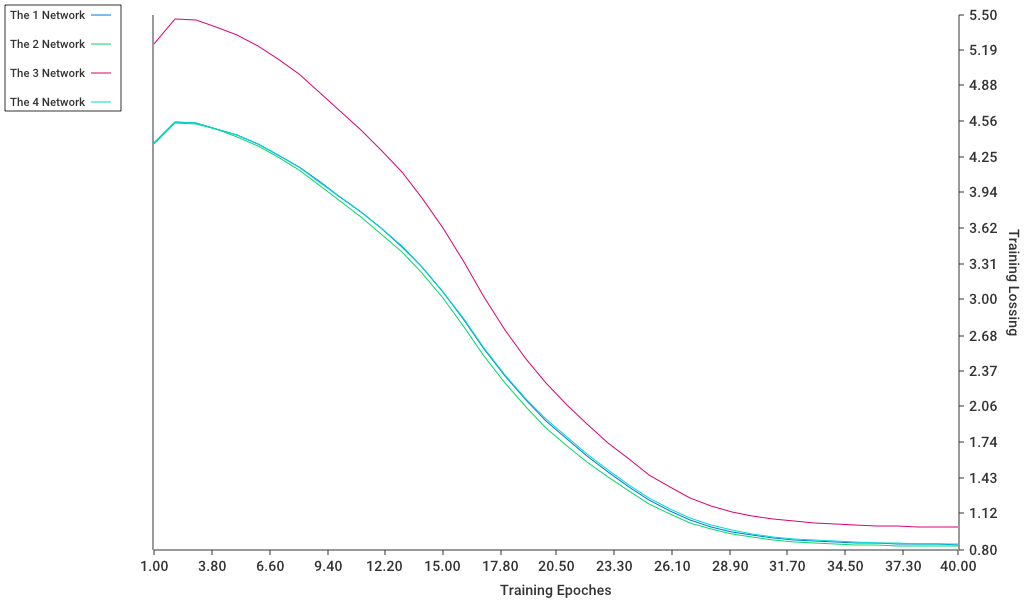
\includegraphics[width=.9\linewidth]{./png/intelImage_subset_allreduce_loss.png}
\end{center}
Allreduce loss (14000 images)
\begin{center}
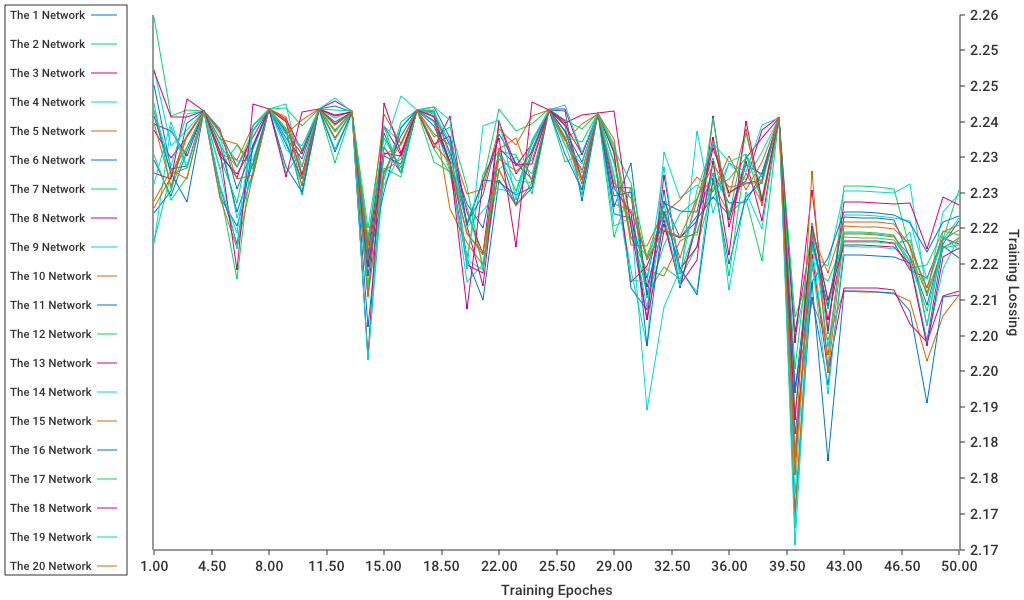
\includegraphics[width=.9\linewidth]{./png/intelImage_allreduce_loss.png}
\end{center}
\end{block}
\end{column}
\end{columns}
\end{frame}
\begin{frame}[label={sec:orgfdf6a46}]{Speedup Diagrams}
\begin{columns}
\begin{column}{0.6\columnwidth}
\begin{block}{Iris for Allreduce and Send\&Recv with different nodes}
\begin{center}
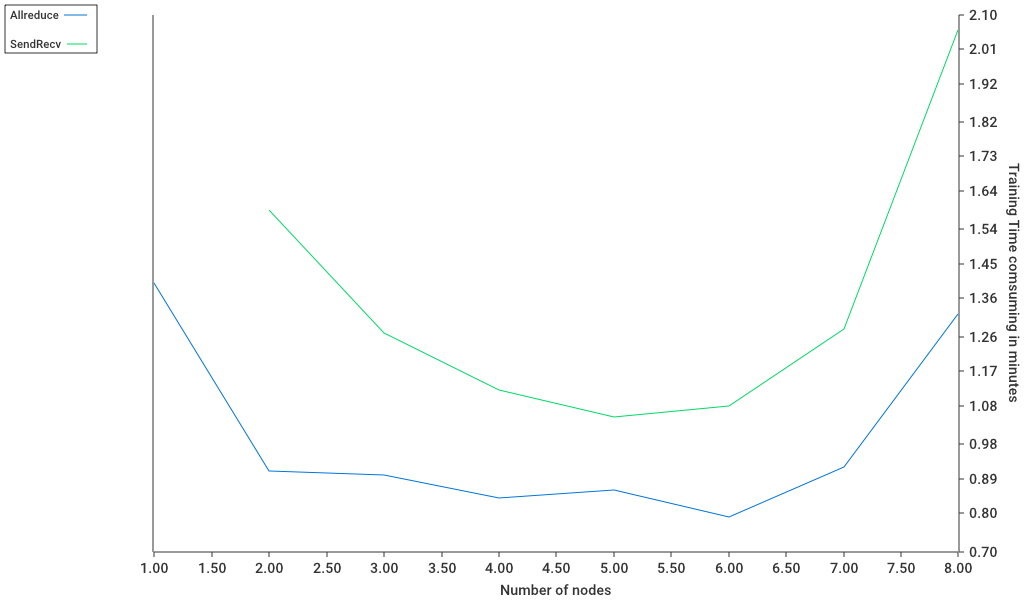
\includegraphics[width=.9\linewidth]{./png/irisSpendup.png}
\end{center}
\end{block}
\end{column}
\begin{column}{0.6\columnwidth}
\begin{block}{Intel Image Classification for Allreduce and Send\&Recv with different nodes}
\begin{center}
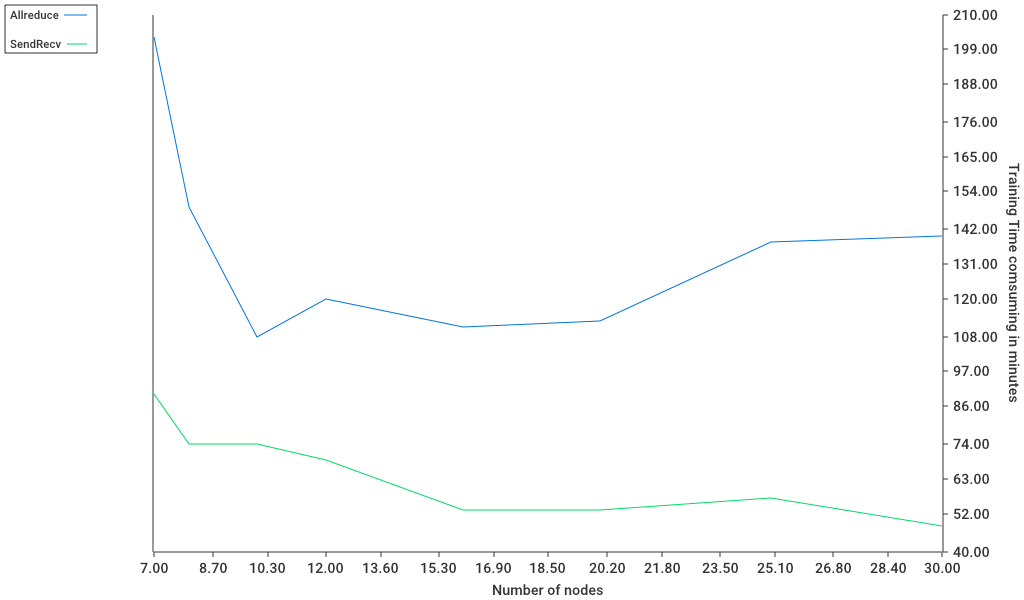
\includegraphics[width=.9\linewidth]{./png/intelImageSpendup.png}
\end{center}
\end{block}
\end{column}
\end{columns}
\end{frame}
\begin{frame}[label={sec:org1ae9f9f}]{Discussion}
\textbf{neural network model implement is not perfect, so the accuracy performance not so well}

\textbf{For each epoch:}
\begin{itemize}
\item Allreduce: about 2 minutes
\item Send\&Recv: about 3.6 minutes, because of synchronization of each batch training
\end{itemize}


\textbf{Change nodes, scaling behavior, such as speedup diagrams is missing}

\textbf{Change the batchsize, reducing mpi communication}
\end{frame}

\begin{frame}[label={sec:org874bfce}]{Conclusion}
\begin{itemize}
\item Golang can also be used for parallel computing
\item neural network implementation of golang can be improved
\item HPC cluster for distributed learning has significant benefits for large dataset
\end{itemize}
\end{frame}
\end{document}